%
% File ucca_parsing.tex
%

\documentclass[11pt]{article}
\usepackage{acl2016}
\usepackage{times}
\usepackage{url}
\usepackage{latexsym}
\usepackage{subfigure}
\usepackage{pgfplotstable}
\usepackage[]{algorithm2e}
\usepackage{hyperref}
\usepackage{color}
\usepackage{lipsum,adjustbox}
\usepackage{tikz}
\usepackage{tikz-dependency}
\usetikzlibrary{shapes,fit,calc,er,positioning,intersections,decorations.shapes,mindmap,trees}
\tikzset{decorate sep/.style 2 args={decorate,decoration={shape backgrounds,shape=circle,shape size=#1,shape sep=#2}}}

\newcommand{\oa}[1]{\footnote{\color{red} #1}}
\newcommand{\daniel}[1]{\footnote{\color{blue} #1}}
\newcommand{\com}[1]{}
\newcommand{\secref}[1]{Section \ref{#1}}
\newcommand{\figref}[1]{Figure~\ref{#1}}
\newcommand{\tabref}[1]{Table~\ref{#1}}

%\aclfinalcopy % Uncomment this line for the final submission
%\def\aclpaperid{***} %  Enter the acl Paper ID here

% To expand the titlebox for more authors, uncomment
% below and set accordingly.
% \addtolength\titlebox{.5in}    

\newcommand\BibTeX{B{\sc ib}\TeX}


\title{Broad-Coverage Semantic Constituency Parsing: \\
A Transition-Based Approach}
  %General Transition-Based Broad-Coverage Semantic Parsing

\author{Daniel Hershcovich \and Omri Abend \and Ari Rappoport \\
  Institute of Computer Science \\
  Hebrew University of Jerusalem \\
  {\tt \{danielh,oabend,arir\}@cs.huji.ac.il}
}

\date{}


\begin{document}
\maketitle

%%%%%%%%%%%%%%%%%%%%%%%%%%%%%%%%%%%%%%%%%%%%%%%%%%%%%%%%%%%%%%%
%%%%%%%%%%%%%%%%%     Abstract
%%%%%%%%%%%%%%%%%%%%%%%%%%%%%%%%%%%%%%%%%%%%%%%%%%%%%%%%%%%%%%%
\begin{abstract}

  Representing many common semantic phenomena requires more expressive formalisms
  than those commonly used for syntactic parsing, motivating research into
  more formally expressive parsers.
  Recent work has focused on broad-coverage semantic parsing into dependency
  (i.e., word-to-word) or abstract (i.e., not grounded in the words and phrases of
  the sentence) representations.
  Instead, we advocate a constituency-based formulation of the
  task and define the broad-coverage constituency semantic parsing task
  (henceforth, {\it BCSP}) using the UCCA semantic scheme and annotated corpora as a testbed.
  We note that there are no existing methods for constituency DAG parsing,
  and propose two transition-based approaches to tackle it:
  (1) creating conversion tools for converting UCCA structures into related
  formalisms and back, and using existing state-of-the-art parsers for
  these settings, and (2) constructing a novel parser for the task.
  
  %We experiment with two types of semantic representations, obtaining
  %encouraging results.
  %Universal Conceptual Cognitive Annotation (UCCA) is a semantic grammatical scheme
  % that assigns 
  %a complete structure to natural language text. We present the first automatic
  % UCCA parser, 
  % a transition-based parser using a novel transition system. We compare the
  % results to baselines 
  % obtained by converting UCCA to CoNNL-X, and training syntactic parsers on the
  % converted dependency trees.
  
\end{abstract}



%%%%%%%%%%%%%%%%%%%%%%%%%%%%%%%%%%%%%%%%%%%%%%%%%%%%%%%%%%%%%%%
\section{Introduction}

% (1) there has been much interest lately in broad-coverage semantic parsing.
%  (2) semantic parsing requires the development of new parsing technology
% (beyond syntactic parsers), as they are formally different. importantly, they
%  are not trees, but DAGs (e.g., argument sharing in control structures;
% see Oepen et al., 2015, AMR).

The formal constraints imposed by available statistical parsers are too restrictive
broad-coverage semantic parsing \cite{oepen2015semeval}.
For instance, arguments that are shared
between predicates are generally represented as multi-parented nodes,
yielding DAG, rather than tree structures. This has motivated much recent
inquiry into semantic parsing with more expressive formalisms.

Earlier work on statistical broad-coverage semantic parsing has mostly
concentrated on shallow semantic analysis, focusing on verb argument structure phenomena.
Recently work has focused on parsing into a more elaborate representation, accounting
for other phenomena, such as inter-clause relations and non-verbal predicates.
Much recent interest has been placed on parsing sentences into abstract meaning representations,
not grounded in the words and phrases, notably AMR \cite{banarescu2013abstract}.
While sharing much of these works' motivation, AMR poses difficulties as it conflates
a wide variety of linguistic phenomena into a single unlayered representation.
Moreover, not grounding the text within the semantic representation,
requires that the alignment between words and logical symbols be automatically
(and imprecisely) detected, and may consequently complicate the parsing task.

An alternative line of work tackles parsing into grounded semantic representations.
Most work of this strand represented semantics using dependency structures.
Various methods have been systematically explored
in two recent SemEval shared tasks \cite{oepen2014semeval,oepen2015semeval}.
Bi-lexical dependencies are indeed an appealing means for representing semantics, partly due to
their structural and conceptual simplicity and the strong and efficient
methods they allow for (see \secref{sec:related}).
However, the assumption that each semantic unit has a unique head is
problematic for representing several frequent constructions which have no clear
head, such as coordination, prepositional phrases and multi-word expressions,
leading to unsystematic treatment of these cases, which yields both conceptual
and practical problems \cite{schwartz2011neutralizing,Ivanova2012who,tsarfaty2012cross}.

In this work we define and tackle the constituency-based semantic parsing task.
Constituency semantic representation is motivated both as it does not
impose the limiting unique head assumption, and its grounding in the text,
which allows for the use of strong and efficient parsing methods.
Indeed, transition-based methods, which have recently produced some of the best
results in syntactic dependency parsing \cite{dyer2015transition,ballesteros2015improved},
can be applied
for constituency parsing as well \cite{sagae2005classifier,zhu2013fast,maier2015discontinuous}. 
We follow the transition-based approach, motivated by its conceptual simplicity,
efficiency and high performance.

We use corpora annotated with the UCCA scheme \cite{abend2013universal} as a test
case\footnote{In fact, while the task definition is not specific to UCCA,
  to the best of our knowledge, these are the only
  semantically annotated corpora that use constituency structures.}
and pursue two complementary parsing strategies.
First, in order to assess the ability of existing technology to tackle the task,
we build converters between the UCCA annotation and two related formalisms:
CoNLL-style dependencies and discontiguous constituency trees.
We are not aware of any statistical constituency DAG parsers, and specifically not
ones that support discontiguous constituents, as required for a broad-coverage semantic
parser (see, e.g., \cite{pitler2015linear,maier2015discontinuous}, for parsers motivated by discontiguous units). Therefore, the conversion is necessarily lossy, but, as we show, is still effective
in practice (\secref{sec:conversion_approach}).
Second, we present a novel transition-based
constituency DAG parser that supports both discontiguous constituents (\secref{sec:direct_approach}). 
We apply the parser both to an in-domain and out-of-domain
scenario, with encouraging results.\oa{are they encouraging?}

%A general parser for this setting must support the prediction of multiple parents,
%as well as of discontiguous constituents, both pervasive phenomena in semantic
%structures even in English (see \secref{sec:data}.
%Multiple parents show up frequently in the context of argument
%sharing, where a certain argument participates in several relations but is only mentioned once.
%Common examples are coordination structures
%(e.g., in ``John went home and took a shower'', ``John'' is an argument of both ``went'' and ``took'')
%or nominalizations (e.g., ``After graduation, John moved to London'', where ``John'' is an argument
%of both ``graduation'' and ``moved'').
%Discontiguous units are common even in syntactic structures in some languages (e.g., German, Bulgarian,
%Korean and many others \cite{kallmeyer2013data}), and can even be found in English, e.g., in reported
%speech: ``'The dog', John said, 'is back again''', and are even more pervasive in English semantic parses
%(see \secref{sec:data}).

The contribution of this work is thus three-fold.
First, we motivate and define the constituency broad-coverage semantic parsing task.
Second, we create converters and assess the ability of existing parsing technology
for formally related settings to address the task, focusing on transition-based methods.
Third, we present the first constituency DAG parser, which is also the
first parser for UCCA. 
All converters, parsers and datasets will be made publicly available upon publication.

%%%%%%%%%%%%%%%%%%%%%%%%%%%%%%%%%%%%%%%%%%%%%%%%%%%%%%%%%%%%%%%
\section{Background}\label{sec:related}

\begin {figure*}
\begin{adjustbox}{width=\textwidth}
  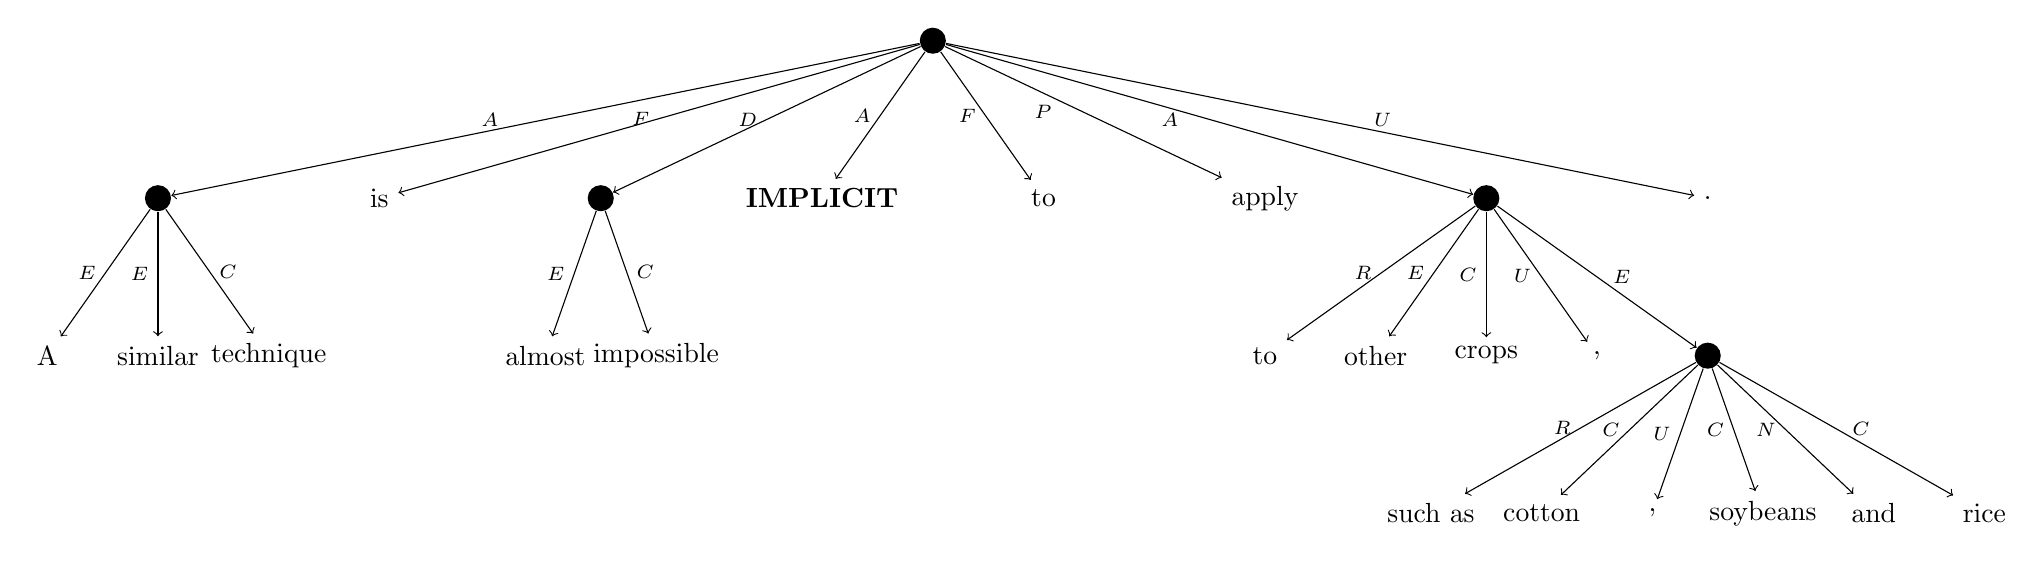
\begin{tikzpicture}[level distance=20mm, ->,
  level 1/.style={sibling distance=8em},
  level 2/.style={sibling distance=4em},
  level 3/.style={sibling distance=4em}]
    \label{fig:similar_technique}
    \node (ROOT) [fill=black, circle] {}
      child {node [fill=black, circle] {}
      {
        child {node {A} edge from parent node[left] {\scriptsize $E$}}
        child {node {similar} edge from parent node[left] {\scriptsize $E$}}
        child {node {technique} edge from parent node[right] {\scriptsize $C$}}
      } edge from parent node[left] {\scriptsize $A\quad$ \hspace{1mm} } }
      child {node {is} edge from parent node[left] {\scriptsize $F$}}
      child {node [fill=black, circle] {}
      {
        child {node {almost} edge from parent node[left] {\scriptsize $E$}}
        child {node {impossible} edge from parent node[right] {\scriptsize $C$}}
      } edge from parent node[left] {\scriptsize $D$} }
      child {node {\textbf{IMPLICIT}} edge from parent node[left] {\scriptsize $A$}}
      child {node {to} edge from parent node[left] {\scriptsize $F$}}
      child {node {apply} edge from parent node[left] {\scriptsize $P\quad$}}
      child {node [fill=black, circle] {}
      {
        child {node {to} edge from parent node[left] {\scriptsize $R$}}
        child {node {other} edge from parent node[left] {\scriptsize $E$}}
        child {node {crops} edge from parent node[left] {\scriptsize $C$}}
        child {node {,} edge from parent node[left] {\scriptsize $U$}}
        child {node [fill=black, circle] {}
        {
          child {node {such as} edge from parent node[left] {\scriptsize $R$}}
          child {node {cotton} edge from parent node[left] {\scriptsize $C$}}
          child {node {,} edge from parent node[left] {\scriptsize $U$}}
          child {node {soybeans} edge from parent node[left] {\scriptsize $C$}}
          child {node {and} edge from parent node[left] {\scriptsize $N$}}
          child {node {rice} edge from parent node[right] {\scriptsize $\; C$}}
        } edge from parent node[right] {\scriptsize $\; E$ \hspace{1mm} } }
      } edge from parent node[left] {\scriptsize $A\;$ \hspace{1mm} } }
      child {node {.} edge from parent node[right] {\scriptsize $\quad \quad U$}}
      ;
  \end{tikzpicture}
\end{adjustbox}
\caption{\label{fig:ucca_example}
  UCCA annotation of the sentence ``A similar technique is almost impossible to
  apply to other crops, such as cotton, soybeans and rice.''.
  The sentence was used by Oepen et al. (2015) to compare between the difference schemes. The sentence includes a single Scene, whose main relation is ``apply'', a secondary relation ``almost impossible'', as well as two complex arguments: ``a similar technique'' and the coordinated argument ``such as cotton, soybeans, and rice''.
}
\end{figure*}

\paragraph{Broad-coverage Deep Semantic Representation.}
The Abstract Meaning Representation (AMR) scheme \cite{banarescu2013abstract},
provides deep semantic annotation in the form of elaborate graphs,
which account for a wider range of predicates, linkage and coreference phenomena.
Formally, it represents sentences as directed graphs, without grounding their
semantic sub-parts in the sentence's words and constituents.

Another line of work that addresses parsing into elaborate semantic structures
is that of Broad-coverage Semantic Dependency Parsing (SDP) \cite{oepen2014semeval,oepen2015semeval}.
Like AMR, SDP also addresses a wide range of argument structures (including verbal, nominal and
adjectival ones) and the inter-relations between them, but uses word-to-word dependency structures.
Three major approaches have been explored:
the Prague Dependency Treebank tectogrammatical layer \cite{bohmova2003prague},
HSPG-derived parsers using the Enju parser\footnote{See \url{http://kmcs.nii.ac.jp/enju/}.},
and dependencies derived from the Lingo ERG Minimal Recursion Semantics represenations \cite{Flic:02}.

Taking a constituency-based approach to semantic parsing,
we use the annotated UCCA corpora, a broad-coverage semantic annotation scheme,
which focuses on predicate-argument structures (verbal, nominal, adjectival and others)
and the inter-relations between them. UCCA \cite{abend2013universal} builds on an established
framework for typological description, ``Basic Linguistic Theory''
\cite{Dixon:10b,Dixon:10a,Dixon:12}, as well as on the Cognitive Linguistics literature. The scheme
has been shown to support rapid annotation and to be semantically stable in translation: UCCA
annotations of translated text usually contain the same set of relationships
\cite{sulem2015conceptual}.

Formally, a UCCA structure is a constituency DAG, whose leaves (or a subset of them) correspond to the words of the text. The nodes of the graph, called ``units'', are either terminals or several elements (not necessarily contiguous) jointly viewed as a single entity according to some semantic or cognitive consideration. The edges bear a category, indicating the role of the sub-unit in the relation that the parent represents. 
The most basic notion is the ``Scene'', which describes a movement, an action or a state.
Each Scene contains one main relation, or anchor, as well as one or more participants. 
For example, the sentence ``After graduation, John moved to Paris'' contains two Scenes, whose main relations are ``graduation'' and ``moved''. The participant ``John'' is a part of both Scenes, while ``Paris'' only of the latter. Further categories account for relations between Scenes and the internal structures of complex arguments (e.g., coordination) and relations (e.g., complex adverbials, such as ``very clearly'').
\figref{fig:ucca_example} presents another example of a UCCA-annotated sentence. 

\paragraph{Related Semantic and Syntactic Parsing Work.}
Semantic parsing methods can be largely partitioned into grammar-based and grammarless methods.
Within the grammar-based literature, most work relied on Combinatory Categorial Grammar (CCG)
\cite{Steedman:00}, which allows to compute semantic structure compositionally from the
syntactic derivations. Notable examples include the Boxer parser \cite{bos2005towards}
and the AMR parser 
by \newcite{artzi2015broad}. Other examples include parsing with Hyperedge Replacement Grammars
\cite{jones2012semantics,chiang2013parsing,peng2015synchronous} and
graph grammars \cite{koller2015semantic}.
A different line of work takes a discriminative, grammarless approach,
pursuing either graph-based methods that predict the highest ranking graph
(tree or DAG) that satisfies a given set of constraints (e.g., \newcite{flanigan2014discriminative}
for AMR parsing)
or a transition-based method that builds the parse incrementally following a series of local
decisions \cite[and much subsequent work]{Nivre03anefficient}.

Despite the greediness\daniel{is beam search greedy too?} and simplicity of transition-based methods, they have yielded excellent
results in a variety of parsing tasks. Within syntactic dependencies parsing, transition-based methods
have been successfully applied to corproa in many languages and domains, yielding some
of the best reported results on this core task \cite{dyer2015transition,ballesteros2015improved}. 
The approach has also yielded results comparable with the state-of-the-art when applied
to constituency parsing \cite{sagae2005classifier,zhu2013fast}, and has been recently extended to
discontiguous constituency parsing \cite{maier2015discontinuous},
yielding improvements over in the parsing of discontiguous constituents in German.
Transition-based parsers have also been developed for dependency DAG structures
\cite{sagae2008shift,tokgoz2015transition}, including a transition-based parser for transforming
syntactic dependencies into AMR parses \cite{wang2015transition}.
Nevertheless, to our knowledge no statistical parser has
been constructed for constituency DAG parsing, a gap which
we address in this work, presenting a transition-based constituency DAG parser that supports
the prediction of discontiguous units.

\oa{Who to compare to? (we take a transition-based approach; later we discuss,
  without comparing, to grammar-based
  or graph-based approaches)
  Constituency parsers that meet some of the criteria: Wolfgang's (all but multiple parents),
        which is state-of-the-art on Negra discontiguous units.
        There are no multiple parent constituency parsers! (so we can't compare)
  Dependency parsers: there are the standard ones (done!), there is MALT non-projective, and there is not MALT with multiple parents. There are other dependency with multiple parents: tokgoez and erdigit (based on earlier work by sagae and tsujii) -- we're trying to get their code.
  
  We'll also say that future work will address other languages, ...
  Evaluation specifically on multiple parents, and on discontiguous.
  Future work: LSTM-version of our parser, conversion from t-layer parsers and such.
}

% ADL comment: I removed these paragraphs because I think the text should zero in on precisely what our research methods, without dwelling on background/ previous work, esp. this early in the text. If this appears at all it should be briefly summarized at the end; say how it informs UCCA, but don't dwell on it.

%Ascribing structure to text or speech is an essential component in any linguistic analysis and computational modeling of language. Large-scale structurally annotated corpora began to emerge in the early 90s, and have made an enormous impact on computational linguistics. 
%Most structurally annotated corpora hitherto focused on formulating a set of distinctions applicable to a certain language or genre. A partial reason for the language specificity of the schemes is that most existing treebanks tend to reflect first and foremost syntactic structures, which vary dramatically between languages. 

%This difficulty has resulted in recent years in two major types of work. 
%One is cross-linguistically applicable {\bf syntactic} representation, much of which is currently addressed under the Universal Dependencies project\footnote{\url{http://universaldependencies.github.io/docs/}}. 
%The other is cross-linguistically applicable {\bf semantic} schemes, expressing a shared level of semantic representation, which are therefore more in line with the purposes of this proposal. The most widely used of these is FrameNet \cite{Fillmore:71}, which focuses on lexical semantics with emphasis on cross-linguistic validity \cite{boas2009multilingual}.
%(though see \cite{goddard2011semantic} for critique). 
%While proving a valuable resource, it has limited coverage, even for English, the most studied language \cite{palmer2010evaluating}, and focuses almost exclusively on argument structure phenomena.

%The Abstract Meaning Representation (AMR) project \cite{AMR:13}, which has attracted considerable attention recently, also provides semantic annotation in the form of elaborate graphs, representing distinctions of various types (including word sense disambiguation, argument structure, compositionality, co-reference). AMR is not optimal for our purposes as it conflates a wide variety of linguistic phenomena into a single unlayered representation, and reflects highly fine-grained phenomena, resulting in many cross-linguistic divergences \cite{XUE14not}.
%AMR poses further difficulties in not embedding the text within the semantic representation, often requires that this correspondence will be automatically (and hence imprecisely) derived.
%(e.g., \cite{flanigan2014discriminative}).

%\subsubsection{Universal Cognitive Conceptual Annotation}

%The inadequacy of string-to-string methods in SMT has resulted in structure aware methods that construe translation as the learning of a function between texts augmented with structural annotation, generally relfecting their syntactic or other structural propoerties. In this sense, imposing linguistic structure on the source and target texts is useful if the translation function between these structures is sufficiently constrained to allow its statistical learning. Semantic representation is an appealing source of cross-linguistically applicable structures, since a major goal of translation is preserving the meaning of the source text.

%UCCA shares AMR's [isn't AMR English-centric?] goal of a cross-linguistically applicable scheme that can benefit semantics-based MT, but is better suited for our purposes in two respects. First, UCCA builds on typological theory and provides empirical support for its cross-linguistic applicability through its application to a sizable corpora in English and French, using the same set of categories \cite{sulem2015conceptual}, in addition to further preliminary experiments in German, Hebrew and Czech. Second, it is built in {\it layers}, each addressing a specific module of semantic distinctions, such as argument-structural, information-theoretic or logical distinctions, which allows more controlled experiments, important in these early stages of semantics-based MT.



%Syntactic dependency trees can in general be non-projective. Graph-based parsers are able to produce such trees, but many transition-based parsers assume projectivity to improve the performance and efficiency of the parser: the number of transitions in such parsers is always $2n$ where $n$ is the number of tokens \cite{nivre2004incrementality}. However, non-projective dependency trees can also be parsed by transition-based parsers in empirical linear time \cite{nivre2009non}.

%In a UCCA graph, labels appear on the edges, whereas nodes are unlabeled. If all the nodes are known, parsing is the same as inducing a graph on them with the correct edge labels. In dependency parsing, a graph is induced on the set of nodes consisting of the tokens in the sentence (and the \textsc{ROOT} symbol). Therefore, it seems that techniques from dependency parsing can be used for UCCA parsing as well.

%\paragraph{Other Semantic Schemes.}

%Although the labels in a UCCA graph are on the edges, it is similar to phrase structure grammar: non-terminal units are internal nodes in the graph, rather than all the edges being between words in the original sentence. In a constituency tree, constituents form a hierarchy above the words of the sentence.

%Methods for constituent parsing can also be useful for UCCA parsing, but the common chart-based approach is also $\mathcal{O}(n^3)$ at best. However, there are also transition-based constituent parsers~\cite{zhu2013fast} with linear run-time complexity.

%Like standard dependency parsers, transition-based constituent parsers are generally unable to produce \textit{discontinuous constituents} (the equivalent of non-projective dependency trees). However, Maier~\shortcite{maier2015discontinuous} introduced a transition-based constituent parsing with a \textsc{swap} transition to allow discontinuous parsing.\footnote{https://github.com/wmaier/uparse}


\subsection{Semantic Constituency Parsing}

A \textit{semantic constituency graph} $G=(V,E)$ over a sequence of tokens $w_1, \ldots, w_n$ is a directed acyclic graph (DAG), where for each $w_i$ ($i=1, \ldots, n$) there exists $t_i \in V$ such that $t_i$ has no children: there is no edge $(t_i, v)$ for any $v \in V$.


%%%%%%%%%%%%%%%%%%%%%%%%%%%%%%%%%%%%%%%%%%%%%%%%%%%%%%%%%%%%%%%
\section{Conversion-based Parsing}\label{sec:conversion_approach}

To our knowledge, no DAG constituency parser currently exists. Therefore, as a first attempt, we use state-of-the-art parsers for existing schemes, and evaluate them on converted data. Since the target schemes are more restrictive, the conversion is necessarily lossy. The accuracy of this method is bounded by the conversion accuracy.
The semantic constituency parsers obtained this way are composed of three steps:
\begin{enumerate}
\item Semantic constituency graphs are converted to the parser's target representation
\item The parser is trained on the converted graphs, and applied to new input using the trained model
\item The output is converted to semantic constituency graphs
\end{enumerate}
Graphs produced by this method for test data is then compared to the gold annotation.
We also perform oracle experiments, where instead of a trained parser's output we use the gold annotation itself, converted to the target representation (and then converted back to semantic constituencies).

\subsection{Conversion to dependency trees}

To evaluate dependency parsers in this scheme, we convert the semantic constituency graphs to dependency trees. This involves a constituency-to-dependency conversion process that is similar to what is done in syntactic treebanks (\cite{...}). In addition, the conversion to a tree structure requires pruning edges such that all nodes remain with a single incoming edge, and a single root remains in the graph.

The conversion from constituency graph to dependency tree is shown in Algorithm~\ref{alg:ucca2conll}. For each node $u$, we define the terminal $\mathrm{head}(u)$, by traversing the nodes reachable form $u$ in priority order, until we reach a terminal. The order is determined by the edge labels. For each terminal $t$, let $u=\mathrm{top}(t)$ if $t=\mathrm{head}(u)$ but $t\neq \mathrm{head}(p)$ for all parents $p$ of $u$. If there is more than one such $u$, we select one of them according to the priority order.

\begin{algorithm}
 \KwData{semantic constituency graph $G$}
 \KwResult{dependency tree $T$}
 $V(T) \leftarrow \emptyset$,
 $E(T) \leftarrow \emptyset$\\
 \ForEach{$t \in \mathrm{terminals}(G)$}{
  $u \leftarrow \mathrm{top}(t)$\\
  $p \leftarrow \mathrm{parent}(u)$\\
  $t^\prime \leftarrow \mathrm{head}(p)$\\
  $\ell \leftarrow \ell_G(p, u)$\\
  $V(T) \leftarrow V(T) \cup \{t\}$\\
  $E(T) \leftarrow E(T) \cup \{(t^\prime, t, \ell)\}$\\
 }
 \caption{Conversion from semantic constituency graph to dependency tree}
 \label{alg:ucca2conll}
\end{algorithm}

The conversion from dependency tree to constituency graph is shown in Algorithm~\ref{alg:conll2ucca}. We define $\mathrm{label}(u)$ heuristically.

\begin{algorithm}
 \KwData{dependency tree $T$}
 \KwResult{semantic constituency graph $G$}
 $r \leftarrow Node()$\\
 $V(G) \leftarrow \{r\}$,
 $E(G) \leftarrow \emptyset$\\
 \ForEach{$t \in V(T)$}{
  $u \leftarrow Node()$\\
  $V(G) \leftarrow V(G) \cup \{t, u\}$\\
  $E(G) \leftarrow E(G) \cup \{(u, \textsc{Terminal}, t\}$\\
  \eIf{$\ell_T(t) = \textsc{Root}$}{
   $E(G) \leftarrow E(G) \cup \{(r, \mathrm{label}(u), u\}$\\
  }{
   $p \leftarrow \mathrm{preterminal}(\mathrm{parent}(t))$\\
   $E(G) \leftarrow E(G) \cup \{(p, \mathrm{label}(u), u\}$\\
  }
 }
 \caption{Conversion from dependency tree to semantic constituency graph}
 \label{alg:conll2ucca}
\end{algorithm}

\subsection{Parsing using dependency parsers}

In order to provide a baseline for UCCA parsing, we trained two state-of-the-art dependency parsers on a dataset resulting from conversion of the UCCA corpus to CoNLL-X format. Then we ran the resulting parser models, converted the results to the UCCA format, and evaluated using the labeled F1, unlabeled F1 and weakly labeled F1 measures. The results are shown in Table~\ref{table:convert}.

%\subsection{Conversion to dependency DAG}
%
%TODO: convert to (projective) dependency DAG
%
%\subsection{Parsing using DAG parsers}
%
%TODO: use Tokg\"oz and Eryi\u{g}it's parser to parse converted DAGs \cite{tokgoz2015transition}

\subsection{Conversion to constituency tree}

Another common format is constituency trees. Here, the conversion is relatively simple: we just remove remote and linkage edges, and all linkage and implicit nodes. This results in a tree that can be parsed by constituency parsers.

\subsection{Parsing using constituency parsers}

The conversion results in constituency trees, but some of the nodes may have a discontinuous yield. Most transition-based parsers are unable to deal with such trees, but we used \textsc{uparse} \cite{maier2015discontinuous}, which is able to parser discontinuous structures. The results are shown in Table~\ref{table:convert}.

%%%%%%%%%%%%%%%%%%%%%%%%%%%%%%%%%%%%%%%%%%%%%%%%%%%%%%%%%%%%%%%
\section{Constituency DAG Parsing}\label{sec:direct_approach}

\subsection{Task definition}

Assuming a pre-defined set $L$ of edge tags, a \textit{UCCA graph} for a text $x=w_1 \ldots w_n$ is a directed graph $G=(V,E)$, where:
\begin{enumerate}
 \item $V$ is a set of nodes s.t. $\{w_1, \ldots, w_n\} \subseteq V$,
 \item $E \subseteq V \times L \times V$ is a set of labeled edges.
\end{enumerate}
The set $V$ of nodes consists of the \textit{terminal} nodes $w_1, \ldots, w_n$, and the non-terminal nodes. The set $E$ of edges is a set of triplets $(u, \ell, v)$, where $u$ and $v$ are nodes and $\ell$ is an edge tag.

In UCCA parsing, $x$ is given and the task is to build $G$.

\subsection{Transition-based UCCA parser}

Many approaches could be used to create a parser for UCCA, such as the graph-based approach
employed in JAMR~\cite{flanigan2014discriminative}.
We chose to adopt the transition-based approach for parsing UCCA.

We define a transition system for UCCA parsing as a quadruple $S=(C,T,c_s,C_t)$, where
\begin{enumerate}
 \item $C$ is a set of configurations.
\end{enumerate}

Our parser architecture combines transition-based constituency parsers \cite{zhu2013fast,maier2015discontinuous} with transition-based DAG dependency parsers \cite{sagae2008shift,tokgoz2015transition}:

\begin{itemize}
	\item Parsing starts with the root node on the stack.
	\item \textsc{Node$_X$} creates a new node on the buffer head as a parent of the first element on the stack (with edge tag $X$), but it does not reduce the first element on the stack; since nodes in UCCA may have multiple parents, they should only be reduced after all their edges have been created.
	\item \textsc{Left-Edge$_X$} and \textsc{Right-Edge$_X$} create a new edge between the first two elements on the stack, but again, they do not reduce any of them, to allow for multiple parents.
	\item \textsc{Left-Remote$_X$} and \textsc{Right-Remote$_X$} are identical to \textsc{Left-Edge$_X$} and \textsc{Right-Edge$_X$}, except that the edges they create are marked as remote. In UCCA there may be long-distance edges, called remote edges.
	\item \textsc{Implicit$_X$} is identical to \textsc{Node$_X$} action, except that the node created by it becomes the child of the stack top rather than its parent, and is marked implicit. Some non-terminal units are implicit units, meaning they do not correspond to any terminals. We add the constraint that implicit nodes cannot have any children.
\end{itemize}

The transitions are:

\textsc{Node$_X$, Implicit$_X$, Left-Edge$_X$, Right-Edge$_X$, Left-Remote$_X$, Right-Remote$_X$, Reduce, Shift, Swap, Finish}

\subsection{Constraints}
Each action has a set of constraint that must be met for that action to be possible. If any of the constraint is not met, the parser may not take that action. The constraints are:
\begin{description}
	\item[\textsc{Finish}] the root node has at least one child.
	\item[\textsc{Shift}] buffer is not empty.
	\item[\textsc{Node$_X$}] stack is not empty, $s_0$ is not the root node, and $X$ is T iff $s_0$ is a terminal.
	\item[\textsc{Implicit$_X$}] stack is not empty, and $s_0$ is not a terminal and not an implicit node.
	\item[\textsc{Reduce$_X$}] stack is not empty, and if $s_0$ is the root node, it has at least one child.
	\item[\textsc{Left-Edge$_X$}] stack has at least two elements, $s_0$ is not a terminal, $s_1$ is not the root node, $s_0$ is not the root node if $s_1$ is a terminal, the edge does not already exist, and $X$ is T iff $s_1$ is a terminal.
	\item[\textsc{Right-Edge$_X$}] stack has at least two elements, $s_1$ is not a terminal, $s_0$ is not the root node, $s_1$ is not the root node if $s_0$ is a terminal, the edge does not already exist, and $X$ is T iff $s_0$ is a terminal.
	\item[\textsc{Left-Remote$_X$}] stack has at least two elements, $s_0$ is not a terminal, $s_1$ is not the root node, $s_0$ is not the root node if $s_1$ is a terminal, the edge does not already exist, $X$ is T iff $s_1$ is a terminal, $s_0$ has at least one child, and $s_1$ has at least one parent.
	\item[\textsc{Right-Remote$_X$}] stack has at least two elements, $s_1$ is not a terminal, $s_0$ is not the root node, $s_1$ is not the root node if $s_0$ is a terminal, the edge does not already exist, $X$ is T iff $s_0$ is a terminal, $s_1$ has at least one child, and $s_0$ has at least one parent.
	\item[\textsc{Swap}] stack has at least two elements, .
\end{description}

\subsection{Feature representation}
\label{subsec:features}

Fig.~\ref{fig:features} shows the features templates adapted from Maier~\shortcite{maier2015discontinuous}. $s_i$ and $b_i$ stand for the $i$th stack and buffer items respectively, $w$ stands for the head word (see~\ref{subsec:head_rules}), $t$ for its POS tag, $e$ for the head incoming edge label. Note that $e$ replaces $c$ (consituent label) from Maier~\shortcite{maier2015discontinuous}, since in UCCA the labels are on the edges rather than the units; and a unit may have more than one incoming edge. $l$ and $r$ ($ll$ and $rr$) represent the leftmost and rightmost children (grand-children) of the element; $u$ handles the unary case.
Concerning the separator features, $p$ is a unique separator feature between the head words of $s_0$ and $s_1$; $q$ is the count of any separator features between them.
$x$ denotes the gap type of a subgraph. There are three possible values, either "none" (fully continuous), "pass" (there is a gap at the root, i.e., this gap must be filled later further up in the graph), or "gap" (the root of this graph fills a gap, i.e., its children have gaps, but the root does not). Finally, $y$ is the sum of all gap lengths.

Fig.~\ref{fig:new_features} shows the features templates introduced in this work. $P$ stands for the number of parents a node currently has, and $C$ for the number of children.

% FEATURES
\begin{figure}[t]
\begin{description}
	\item[unigrams] \hfill \\
	$s_0te, s_0we, s_1te, s_1we, s_2te, s_2we, s_3te, s_3we,$ \\
	$b_0wt, b_1wt, b_2wt, b_3wt,$ \\
	$s_0lwe, s_0rwe, s_0uwe, s_1lwe, s_1rwe, s_1uwe$
	\item[bigrams] \hfill \\
	$s_0ws_1w, s_0ws_1e, s_0es_1w, s_0es_1e, s_0wb_0w, s_0wb_0t,$ \\
	$s_0eb_0w, s_0eb_0t, s_1wb_0w, s_1wb_0t, s_1eb_0w, s_1eb_0t,$ \\
	$b_0wb_1w, b_0wb_1t, b_0tb_1w, b_0tb_1t$
	\item[trigrams] \hfill \\
	$s_0es_1es_2w, s_0es_1es_2e, s_0es_1eb_0w, s_0es_1eb_0t,$ \\
	$s_0es_1wb_0w, s_0es_1wb_0t, s_0ws_1es_2e, s_0ws_1eb_0t$
	\item[extended] \hfill \\
	$s_0llwe, s_0lrwe, s_0luwe, s_0rlwe, s_0rrwe,$ \\
	$s_0ruwe, s_0ulwe, s_0urwe, s_0uuwe, s_1llwe,$ \\
	$s_1lrwe, s_1luwe, s_1rlwe, s_1rrwe, s_1ruwe$
	\item[separator] \hfill \\
	$s_0wp, s_0wep, s_0wq, s_0wcq, s_0es_1ep, s_0es_1eq,$ \\
	$s_1wp, s_1wep, s_1wq, s_1weq$
	\item[\textsc{Disco} unigrams] \hfill \\
	$s_0xwe, s_1xwe, s_2xwe, s_3xwe,$ \\
	$s_0xte, s_1xte, s_2xte, s_3xte,$ \\
	$s_0xy, s_1xy, s_2xy, s_3xy$
	\item[\textsc{Disco} bigrams] \hfill \\
	$s_0xs_1e, s_0xs_1w, s_0xs_1x, s_0ws_1x, s_0es_1x,$ \\
	$s_0xs_2e, s_0xs_2w, s_0xs_2x, s_0ws_2x, s_0es_2x,$ \\
	$s_0ys_1y, s_0ys_2y, s_0xb_0t, s_0xb_0w$
\end{description}
\caption{Feature Templates}
\medskip
\small
Feature from \cite{maier2015discontinuous}.
$s_i$, $b_i$: stack and buffer items.
$w$: head word. $t$: POS tag.
$e$: main incoming edge label.
$l$, $r$ ($ll$, $rr$): leftmost and rightmost children (grand-children).
$u$ ($uu$): unary child (grandchild).
$p$: unique separator between $s_0$ and $s_1$.
$q$: separator count.
$x$: gap type.
$y$: sum of gap lengths.
\label{fig:features}
\end{figure}

% NEW FEATURES
\begin{figure}[t]
\begin{description}
	\item[degree] \hfill \\
	$s_0P, s_0C$
\end{description}
\caption{New Feature Templates}
\medskip
\small
Feature introduced in this work.
\label{fig:new_features}
\end{figure}

\subsection{Head rules}
\label{subsec:head_rules}

The following rules were used to determine the head of a unit.

%%%%%%%%%%%%%%%%%%%%%%%%%%%%%%%%%%%%%%%%%%%%%%%%%%%%%%%%%%%%%%%
\section{Data}\label{sec:data}

Give examples of cases where multiple parents and/or discontiguous units show up.

\oa{put statistics here similar to table 1 in the semeval 2015 paper; specifically, treewidth may be interesting}

\begin{table}[ht]
\begin{tabular}{lccc}
Node type & count & \% multiple parents & \% discontinuous \\
\hline
All &  & \\
Foundational &  & \\
Non-terminals &  & \\
Terminals &  &
\end{tabular}
\caption{Quantitative characterization of structure in the UCCA corpus. 
}
\end{table}

We should give some statistics about the pervasiveness of discontiguities and multiple parents in our corpora.

%%%%%%%%%%%%%%%%%%%%%%%%%%%%%%%%%%%%%%%%%%%%%%%%%%%%%%%%%%%%%%%
\section{Results}

Table~\ref{table:convert} shows the results.
\begin{table*}
\pgfplotstabletypeset[col sep=comma,
     columns={Method,LAS,LAS (sentences),UAS,UAS (sentences),labeled F1,labeled F1 (sentences),unlabeled F1,unlabeled F1 (sentences),weak labeled F1,weak labeled F1 (sentences)},
     columns/Method/.style={string type, column type=l,
         postproc cell content/.code={%
             \pgfplotsutilstrreplace{_}{\_}{##1}%
             \pgfkeyslet{/pgfplots/table/@cell content}\pgfplotsretval
         },}
    ]{results.csv}
\caption{Results of Conversion and Annotation using Dependency Parsers}
\label{table:convert}
\end{table*}

%%%%%%%%%%%%%%%%%%%%%%%%%%%%%%%%%%%%%%%%%%%%%%%%%%%%%%%%%%%%%%%
\section{Conclusion}

We have presented a transition-based parser for UCCA, which is a semantic 

Future work:
\begin{itemize}
\item \textsc{smatch} for scoring
\item find the best conversion rules automatically
\end{itemize}

\bibliography{references}
\bibliographystyle{acl2016}

\end{document}


\com{
  (8) we expriment with the UCCA corpus...
  (7) since this is the first parser for the task, we compare the results to partial
  implementations of the algorithm. we also conduct a comparison with existing parsers for similar
  parsing tasks.
  (9) our contribution: \#1 defining the 
  \#2 first parser for broad-coverage consituency-based parsing; \#3 first parser for UCCA;
  Previous work: the work has interesting connections to syntactic parsing, to SRL (which also has both dependency
  and constituency versions), and to semantic parsing into logical forms, but is different from the,
  see discussion in (Oepen et al., 2015). Also AMR parsing.

Universal Conceptual Cognitive Annotation (UCCA) is a recently introduced semantic annotation scheme. It takes a semantic approach to grammatical representation, describing relations between words and phrases in natural language text. The foundational layer can potentially be extended by any number of additional layers to provide refinements to the existing scheme, but it already covers many of the basic semantic relations in language. The annotation is represented as a directed acyclic graph (DAG), where edges denote semantic dependencies between abstract units. UCCA can be easily annotated manually without expert knowledge in linguistics, making it attractive as a resource for semantic tasks---an alternative to syntactic annotation, which is costly. A corpus containing 160K words from the English Wikipedia has been manually annotated~\cite{abend2013universal}.

UCCA exhibits three properties that are generally absent in syntactic schemes:
\begin{description}
\item[Multiple parents.] In general, the UCCA graph is a DAG and not a tree.
\item[Discontinuity.] The yield of a node may have gaps.
\item[Non-terminal units.] There are units representing abstract entities or events, and not all nodes correspond to tokens.
\end{description}

This work is the first attempt at automatic UCCA parsing.
}
